\documentclass[11pt,a4paper]{report}
\usepackage[textwidth=37em,vmargin=30mm]{geometry}
\usepackage{calc,xunicode,amsmath,amssymb,paralist,enumitem,tabu,booktabs,datetime2,xeCJK,xeCJKfntef,listings}
\usepackage{tocloft,fancyhdr,tcolorbox,xcolor,graphicx,eso-pic,xltxtra,xelatexemoji}

\newcommand{\envyear}[0]{2025}
\newcommand{\envdatestr}[0]{2025-04-16}
\newcommand{\envfinaldir}[0]{webdb/2025/20250416/final}

\usepackage[hidelinks]{hyperref}
\hypersetup{
    colorlinks=false,
    pdfpagemode=FullScreen,
    pdftitle={Web Digest - \envdatestr}
}

\setlength{\cftbeforechapskip}{10pt}
\renewcommand{\cftchapfont}{\rmfamily\bfseries\large\raggedright}
\setlength{\cftbeforesecskip}{2pt}
\renewcommand{\cftsecfont}{\sffamily\small\raggedright}

\setdefaultleftmargin{2em}{2em}{1em}{1em}{1em}{1em}

\usepackage{xeCJK,xeCJKfntef}
\xeCJKsetup{PunctStyle=plain,RubberPunctSkip=false,CJKglue=\strut\hskip 0pt plus 0.1em minus 0.05em,CJKecglue=\strut\hskip 0.22em plus 0.2em}
\XeTeXlinebreaklocale "zh"
\XeTeXlinebreakskip = 0pt


\setmainfont{Brygada 1918}
\setromanfont{Brygada 1918}
\setsansfont{IBM Plex Sans}
\setmonofont{JetBrains Mono NL}
\setCJKmainfont{Noto Serif CJK SC}
\setCJKromanfont{Noto Serif CJK SC}
\setCJKsansfont{Noto Sans CJK SC}
\setCJKmonofont{Noto Sans CJK SC}

\setlength{\parindent}{0pt}
\setlength{\parskip}{8pt}
\linespread{1.15}

\lstset{
	basicstyle=\ttfamily\footnotesize,
	numbersep=5pt,
	backgroundcolor=\color{black!5},
	showspaces=false,
	showstringspaces=false,
	showtabs=false,
	tabsize=2,
	captionpos=b,
	breaklines=true,
	breakatwhitespace=true,
	breakautoindent=true,
	linewidth=\textwidth
}






\newcommand{\coverpic}[2]{
    % argv: itemurl, authorname
    Cover photo by #2~~(\href{#1}{#1})
}
\newcommand{\makeheader}[0]{
    \begin{titlepage}
        % \newgeometry{hmargin=15mm,tmargin=21mm,bmargin=12mm}
        \begin{center}
            
            \rmfamily\scshape
            \fontspec{BaskervilleF}
            \fontspec{Old Standard}
            \fontsize{59pt}{70pt}\selectfont
            WEB\hfill DIGEST
            
            \vfill
            % \vskip 30pt
            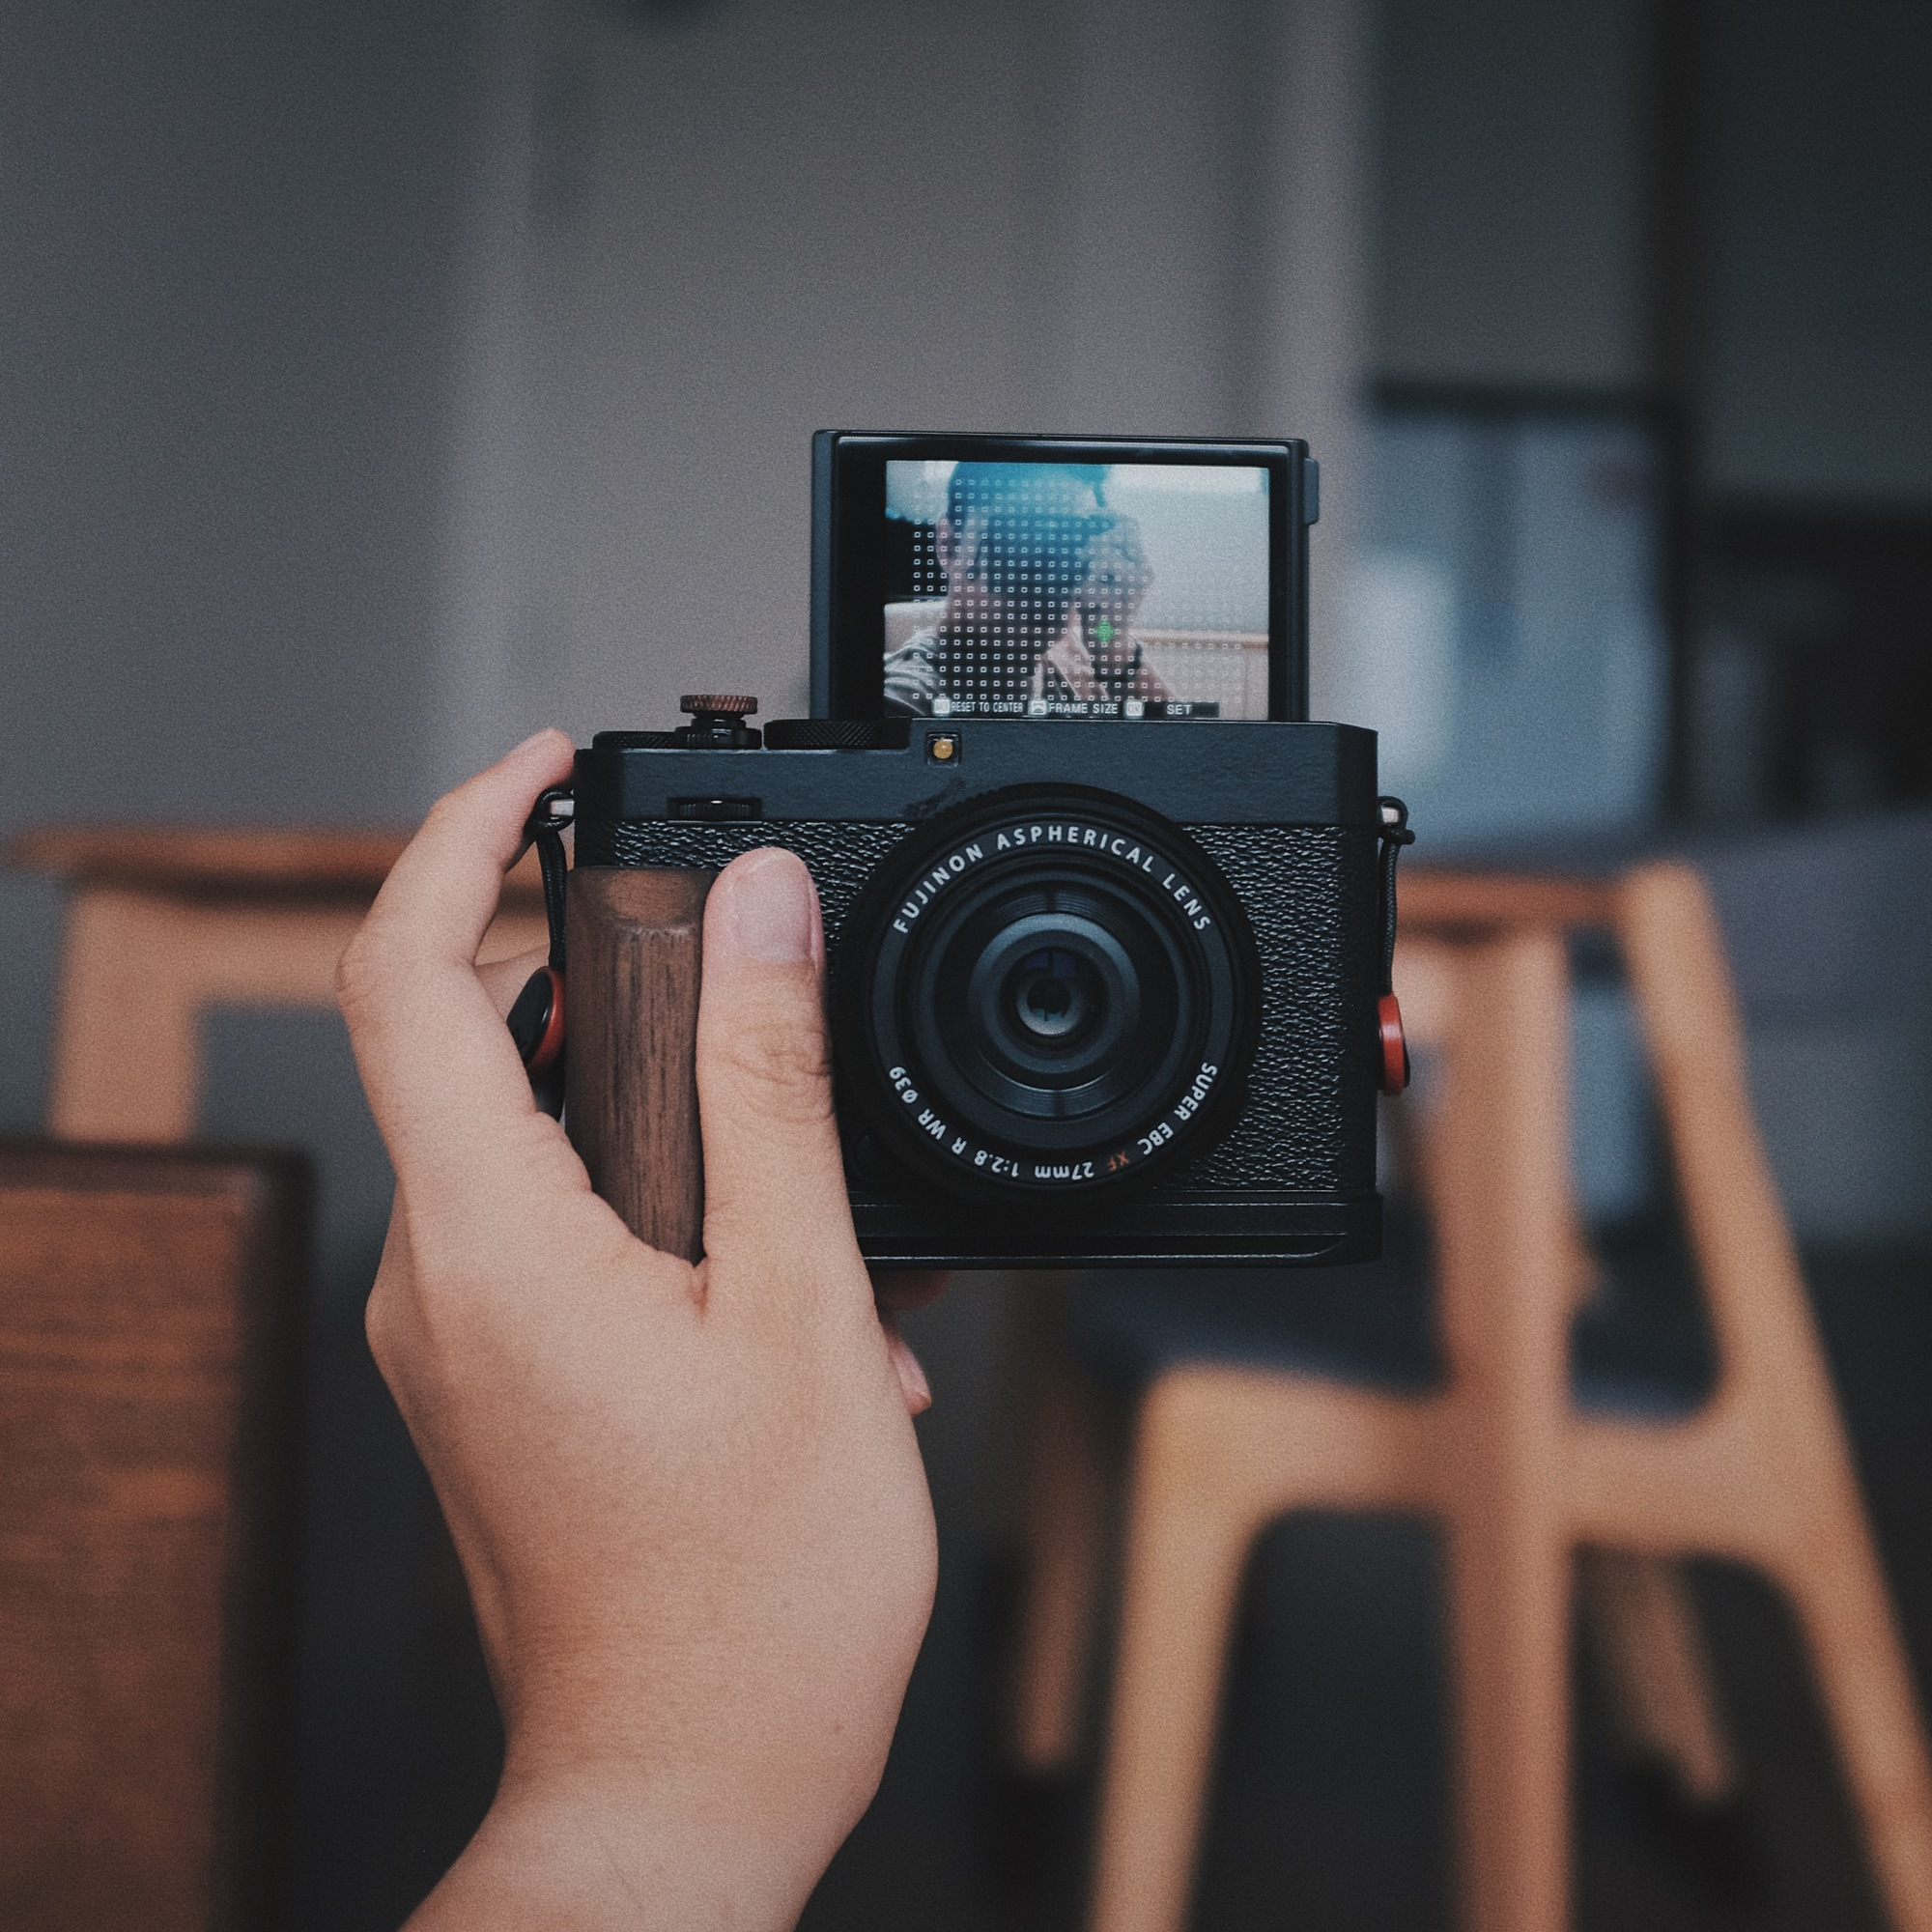
\includegraphics[width=\linewidth]{\envfinaldir/coverpic-prod.jpg}\par
            % \vskip 30pt
            \vfill

            \normalsize\rmfamily\scshape
            \copyright{} The Web Digest Project \hfill\large \envdatestr
        \end{center}
    \end{titlepage}
    % \restoregeometry
}
\newcommand{\simplehref}[1]{%
    \textcolor{blue!80!green}{\href{#1}{#1}}%
}
\renewcommand{\contentsname}{\center\Huge\sffamily\bfseries Contents\par\vskip 20pt}
\newcounter{ipartcounter}
\setcounter{ipartcounter}{0}
\newcommand{\ipart}[1]{
    % \vskip 20pt
    \clearpage
    \stepcounter{ipartcounter}
    \phantomsection
    \addcontentsline{toc}{chapter}{#1}
    % \begin{center}
    %     \Huge
    %     \sffamily\bfseries
    %     #1
    % \end{center}
    % \vskip 20pt plus 7pt
}
\newcounter{ichaptercounter}
\setcounter{ichaptercounter}{0}
\newcommand{\ichapter}[1]{
    % \vskip 20pt
    \clearpage
    \stepcounter{ichaptercounter}
    \phantomsection
    \addcontentsline{toc}{section}{\numberline{\arabic{ichaptercounter}}#1}
    \begin{center}
        \Huge
        \sffamily\bfseries
        #1
    \end{center}
    \vskip 20pt plus 7pt
}
\newcommand{\entrytitlefont}[1]{\subsection*{\raggedright\Large\sffamily\bfseries#1}}
\newcommand{\entryitemGeneric}[2]{
    % argv: title, url
    \parbox{\linewidth}{
        \entrytitlefont{#1}\par\vskip 5pt
        \footnotesize\ttfamily\mdseries
        \simplehref{#2}
    }\vskip 11pt plus 11pt minus 1pt
}
\newcommand{\entryitemGithub}[3]{
    % argv: title, url, desc
    \parbox{\linewidth}{
        \entrytitlefont{#1}\par\vskip 5pt
        \footnotesize\ttfamily\mdseries
        \simplehref{#2}\par\vskip 5pt
        \small\rmfamily\mdseries#3
    }\vskip 11pt plus 11pt minus 1pt
}
\newcommand{\entryitemAp}[3]{
    % argv: title, url, desc
    \parbox{\linewidth}{
        \entrytitlefont{#1}\par\vskip 5pt
        \footnotesize\ttfamily\mdseries
        \simplehref{#2}\par\vskip 5pt
        \small\rmfamily\mdseries#3
    }\vskip 11pt plus 11pt minus 1pt
}
\newcommand{\entryitemHackernews}[3]{
    % argv: title, hnurl, rawurl
    % \parbox{\linewidth}{
    %     \entrytitlefont{#1}\par\vskip 5pt
    %     \footnotesize\ttfamily\mdseries
    %     \simplehref{#3}\par
    %     \textcolor{black!50}{\href{#2}{#2}}
    % }\vskip 11pt plus 11pt minus 1pt
    \begin{minipage}{\linewidth}
            \entrytitlefont{#1}\par\vskip 5pt
            \footnotesize\ttfamily\mdseries
            \simplehref{#3}\par
            \textcolor{black!50}{\href{#2}{#2}}
    \end{minipage}\par\vskip 11pt plus 11pt minus 1pt
}







\begin{document}

\makeheader

\tableofcontents\clearpage




\ipart{Developers}
\ichapter{Hacker News}
\entryitemTwoLinks{What the hell is a target triple?}{https://news.ycombinator.com/item?id=43696756}{https://mcyoung.xyz/2025/04/14/target-triples/}

\entryitemTwoLinks{It's easier than ever to de-censor videos}{https://news.ycombinator.com/item?id=43695701}{https://www.jeffgeerling.com/blog/2025/its-easier-ever-de-censor-videos}

\entryitemTwoLinks{Clolog}{https://news.ycombinator.com/item?id=43695620}{https://github.com/bobschrag/clolog}

\entryitemTwoLinks{Generate videos in Gemini and Whisk with Veo 2}{https://news.ycombinator.com/item?id=43695592}{https://blog.google/products/gemini/video-generation/}

\entryitemTwoLinks{Doge Is Far Short of Its Goal, and Still Overstating Its Progress}{https://news.ycombinator.com/item?id=43693584}{https://www.nytimes.com/2025/04/13/us/politics/doge-contracts-savings.html}

\entryitemTwoLinks{ICE Agents Realize They Arrested Wrong Teen, Say 'Take Him Anyway'}{https://news.ycombinator.com/item?id=43693531}{https://www.newsweek.com/merwil-gutierrez-ice-wrong-teen-el-salvador-2059783}

\entryitemTwoLinks{How to win an argument with a toddler}{https://news.ycombinator.com/item?id=43693402}{https://seths.blog/2025/04/how-to-win-an-argument-with-a-toddler/}

\entryitemTwoLinks{Philosophy Major Snatched by ICE During Citizenship Interview}{https://news.ycombinator.com/item?id=43693375}{https://dailynous.com/2025/04/15/philosophy-major-snatched-by-ice-during-citizenship-interview/}

\entryitemTwoLinks{Hacking the Postgres wire protocol}{https://news.ycombinator.com/item?id=43693326}{https://pgdog.dev/blog/hacking-postgres-wire-protocol}

\entryitemTwoLinks{You cannot have our user's data}{https://news.ycombinator.com/item?id=43692998}{https://sourcehut.org/blog/2025-04-15-you-cannot-have-our-users-data/}

\entryitemTwoLinks{America underestimates the difficulty of bringing manufacturing back}{https://news.ycombinator.com/item?id=43692677}{https://www.molsonhart.com/blog/america-underestimates-the-difficulty-of-bringing-manufacturing-back}

\entryitemTwoLinks{Launch HN: mrge.io (YC X25) – Cursor for code review}{https://news.ycombinator.com/item?id=43692476}{https://news.ycombinator.com/item?id=43692476}

\entryitemTwoLinks{How the U.S. became a science superpower}{https://news.ycombinator.com/item?id=43692360}{https://steveblank.com/2025/04/15/how-the-u-s-became-a-science-superpower/}

\entryitemTwoLinks{Chroma: Ubisoft's internal tool used to simulate color-blindness}{https://news.ycombinator.com/item?id=43692089}{https://github.com/ubisoft/Chroma}

\entryitemTwoLinks{4chan Sharty Hack And Janitor Email Leak}{https://news.ycombinator.com/item?id=43691334}{https://knowyourmeme.com/memes/events/april-2025-4chan-sharty-hack-and-janitor-email-leak}

\entryitemTwoLinks{Whistleblower details how DOGE may have taken sensitive NLRB data}{https://news.ycombinator.com/item?id=43691142}{https://www.npr.org/2025/04/15/nx-s1-5355896/doge-nlrb-elon-musk-spacex-security}

\entryitemTwoLinks{Teuken-7B-Base and Teuken-7B-Instruct: Towards European LLMs (2024)}{https://news.ycombinator.com/item?id=43690955}{https://arxiv.org/abs/2410.03730}

\entryitemTwoLinks{Show HN: Unsure Calculator – back-of-a-napkin probabilistic calculator}{https://news.ycombinator.com/item?id=43690289}{https://filiph.github.io/unsure/}

\entryitemTwoLinks{Show HN: MCP-Shield – Detect security issues in MCP servers}{https://news.ycombinator.com/item?id=43689178}{https://github.com/riseandignite/mcp-shield}

\entryitemTwoLinks{Hacking a Smart Home Device (2024)}{https://news.ycombinator.com/item?id=43688658}{https://jmswrnr.com/blog/hacking-a-smart-home-device}\ichapter{Phoronix}
\entryitemGeneric{\hskip 0pt{}GCC 15 Squeezes In Some Last Minute Adjustments For AMD Zen 5 "znver5"}{https://www.phoronix.com/news/GCC-15.1-Last-Minute-Znver5-Bit}

\entryitemGeneric{\hskip 0pt{}TrueNAS 25.04 Released For Unifying SCALE \& CORE Offerings}{https://www.phoronix.com/news/TrueNAS-25.04-Released}

\entryitemGeneric{\hskip 0pt{}Fedora Server 42 Is Performing Well On 5th Gen AMD EPYC "Turin"}{https://www.phoronix.com/review/fedora-server-42-epyc}

\entryitemGeneric{\hskip 0pt{}Mesa 25.1 Panfrost \& PanVK Begin Supporting Newer Arm Mali 5th Gen Graphics}{https://www.phoronix.com/news/Mesa-25.1-Newer-Mali-5th-Gen}

\entryitemGeneric{\hskip 0pt{}Fedora 42 Released As A Fantastic Update To This Leading-Edge Linux Distribution}{https://www.phoronix.com/news/Fedora-42-Released}

\entryitemGeneric{\hskip 0pt{}Linux Might Drop The Apple HFS / HFS+ File-System Kernel Driver Support}{https://www.phoronix.com/news/Linux-2025-Sad-State-HFS}

\entryitemGeneric{\hskip 0pt{}Intel's VPL GPU Runtime Preparing To Drop The Media SDK With Pre-Tigerlake Support}{https://www.phoronix.com/news/Intel-VPL-GPU-RT-End-Media-SDK}

\entryitemGeneric{\hskip 0pt{}Linux 6.16 Expected To Remove Datagram Congestion Control Protocol "DCCP" Networking}{https://www.phoronix.com/news/Linux-6.16-Net-Next-Drops-DCCP}

\entryitemGeneric{\hskip 0pt{}Manjaro 25.0 Released With Upgrades To Linux 6.12 Plus GNOME 48 \& KDE Plasma 6.3}{https://www.phoronix.com/news/Manjaro-Linux-25.0-Released}\ichapter{Dribbble}
\entryitemGeneric{\hskip 0pt{}Altitude}{https://dribbble.com/shots/25902364-Altitude}

\entryitemGeneric{\hskip 0pt{}Road Tripping}{https://dribbble.com/shots/25900418-Road-Tripping}

\entryitemGeneric{\hskip 0pt{}Lion sketches}{https://dribbble.com/shots/25898381-Lion-sketches}

\entryitemGeneric{\hskip 0pt{}Bloksy Logo Design - City, Colorful, Building, Construction}{https://dribbble.com/shots/25898764-Bloksy-Logo-Design-City-Colorful-Building-Construction}

\entryitemGeneric{\hskip 0pt{}Cute Shiba Catching a Ball}{https://dribbble.com/shots/25900210-Cute-Shiba-Catching-a-Ball}

\entryitemGeneric{\hskip 0pt{}Corti: Visual identity exploration}{https://dribbble.com/shots/25899331-Corti-Visual-identity-exploration}

\entryitemGeneric{\hskip 0pt{}Chat App - Two Pages of Sketches}{https://dribbble.com/shots/25890352-Chat-App-Two-Pages-of-Sketches}

\entryitemGeneric{\hskip 0pt{}Nite Riot®\_Film Production // Case Study\_Vol.2.0}{https://dribbble.com/shots/25889874-Nite-Riot-Film-Production-Case-Study-Vol-2-0}

\entryitemGeneric{\hskip 0pt{}Lock Layer Logo Design - Shield, Letter L, Cube, Security}{https://dribbble.com/shots/25889313-Lock-Layer-Logo-Design-Shield-Letter-L-Cube-Security}

\entryitemGeneric{\hskip 0pt{}Simple vs Advanced}{https://dribbble.com/shots/25890403-Simple-vs-Advanced}

\entryitemGeneric{\hskip 0pt{}🔐 Cybersecurity Mobile App}{https://dribbble.com/shots/25887711--Cybersecurity-Mobile-App}

\entryitemGeneric{\hskip 0pt{}Lion}{https://dribbble.com/shots/25884438-Lion}

\entryitemGeneric{\hskip 0pt{}Hollo Logo Design}{https://dribbble.com/shots/25883411-Hollo-Logo-Design}

\entryitemGeneric{\hskip 0pt{}Adobe Acrobat Logo Redesign Concept}{https://dribbble.com/shots/25884888-Adobe-Acrobat-Logo-Redesign-Concept}

\entryitemGeneric{\hskip 0pt{}Corti: Visual identity exploration}{https://dribbble.com/shots/25871312-Corti-Visual-identity-exploration}

\entryitemGeneric{\hskip 0pt{}Revolve Logo Design}{https://dribbble.com/shots/25885583-Revolve-Logo-Design}

\entryitemGeneric{\hskip 0pt{}Fintech Web Design \& Landing Page for Puzzle}{https://dribbble.com/shots/25652139-Fintech-Web-Design-Landing-Page-for-Puzzle}

\entryitemGeneric{\hskip 0pt{}Monster Pony Wooden toy}{https://dribbble.com/shots/25880300-Monster-Pony-Wooden-toy}

\entryitemGeneric{\hskip 0pt{}Web Design Crypto Trading}{https://dribbble.com/shots/25879747-Web-Design-Crypto-Trading}

\entryitemGeneric{\hskip 0pt{}Educate AI Logo Design - Letter E, Monogram, Education}{https://dribbble.com/shots/25879659-Educate-AI-Logo-Design-Letter-E-Monogram-Education}

\entryitemGeneric{\hskip 0pt{}Polydex}{https://dribbble.com/shots/25879909-Polydex}

\entryitemGeneric{\hskip 0pt{}Greetings from}{https://dribbble.com/shots/25881723-Greetings-from}

\entryitemGeneric{\hskip 0pt{}Kilo Code - Branding}{https://dribbble.com/shots/25881666-Kilo-Code-Branding}

\entryitemGeneric{\hskip 0pt{}Flight Tracking Mobile App UI Design}{https://dribbble.com/shots/25869631-Flight-Tracking-Mobile-App-UI-Design}


\ipart{Developers~~~~(zh-Hans)}
\ichapter{Solidot}
\entryitemGeneric{\hskip 0pt{}日本监管机构要求 Google 停止垄断行为}{https://www.solidot.org/story?sid=81056}

\entryitemGeneric{\hskip 0pt{}美国六大科技巨头被指十年逃避了近 2780 亿美元的公司税}{https://www.solidot.org/story?sid=81055}

\entryitemGeneric{\hskip 0pt{}科学家绘制鸡基因调控的详细图谱}{https://www.solidot.org/story?sid=81054}

\entryitemGeneric{\hskip 0pt{}能随意塑形的流体电池}{https://www.solidot.org/story?sid=81053}

\entryitemGeneric{\hskip 0pt{}Temu 在美国撤下了 Google Shopping 广告}{https://www.solidot.org/story?sid=81052}

\entryitemGeneric{\hskip 0pt{}英特尔以 44.6 亿美元将 Altera 控股权出售给私募}{https://www.solidot.org/story?sid=81051}

\entryitemGeneric{\hskip 0pt{}特朗普政府对哈佛暂停 22 亿美元拨款}{https://www.solidot.org/story?sid=81050}

\entryitemGeneric{\hskip 0pt{}Pinta 3.0 释出}{https://www.solidot.org/story?sid=81049}

\entryitemGeneric{\hskip 0pt{}微软警告 Windows 11 用户不要删除神秘的空文件夹}{https://www.solidot.org/story?sid=81048}

\entryitemGeneric{\hskip 0pt{}中国民航局颁发首批飞行出租车运营合格证}{https://www.solidot.org/story?sid=81047}

\entryitemGeneric{\hskip 0pt{}英国高级警官呼吁禁止 16 岁以下儿童使用社交媒体}{https://www.solidot.org/story?sid=81046}

\entryitemGeneric{\hskip 0pt{}2022 年全球逾 300 万儿童死于抗生素耐药性感染}{https://www.solidot.org/story?sid=81045}

\entryitemGeneric{\hskip 0pt{}4 岁儿童就支持少数服从多数}{https://www.solidot.org/story?sid=81044}

\entryitemGeneric{\hskip 0pt{}傅利叶推出开源人形机器人 Fourier N1}{https://www.solidot.org/story?sid=81043}

\entryitemGeneric{\hskip 0pt{}日本人口连续 14 年减少}{https://www.solidot.org/story?sid=81042}

\entryitemGeneric{\hskip 0pt{}OpenAI API 可能要求客户验证身份 }{https://www.solidot.org/story?sid=81041}

\entryitemGeneric{\hskip 0pt{}AO3 进入了新时代}{https://www.solidot.org/story?sid=81040}

\entryitemGeneric{\hskip 0pt{}乌鸦会几何学}{https://www.solidot.org/story?sid=81039}

\entryitemGeneric{\hskip 0pt{}GitHub 短暂限制中国 IP 访问}{https://www.solidot.org/story?sid=81038}

\entryitemGeneric{\hskip 0pt{}德国 UBI 实验未发现参与者会停止工作}{https://www.solidot.org/story?sid=81037}\ichapter{V2EX}
\entryitemGeneric{\hskip 0pt{}[YouTube] 推荐一个手机上无广告看 YouTube 的 app}{https://www.v2ex.com/t/1125736}

\entryitemGeneric{\hskip 0pt{}[问与答] steam 怎么知道我开了代理?}{https://www.v2ex.com/t/1125734}

\entryitemGeneric{\hskip 0pt{}[NAS] 绿联 NAS UGOS Pro 体验(避坑)}{https://www.v2ex.com/t/1125733}

\entryitemGeneric{\hskip 0pt{}[硬件] 有没有大佬可以做微信群监听采集发布}{https://www.v2ex.com/t/1125732}

\entryitemGeneric{\hskip 0pt{}[互联网] 推荐几个端口打洞的工具试试?}{https://www.v2ex.com/t/1125731}

\entryitemGeneric{\hskip 0pt{}[宽带症候群] 在广州用联通,跟电信比有什么差异}{https://www.v2ex.com/t/1125730}

\entryitemGeneric{\hskip 0pt{}[推广] [Claw] 云服务器 Devbox 是 ClawCloud 新出品的开发容器}{https://www.v2ex.com/t/1125729}

\entryitemGeneric{\hskip 0pt{}[Apple] MBP Mid 2012 13 寸 左 Command+V 问题}{https://www.v2ex.com/t/1125728}

\entryitemGeneric{\hskip 0pt{}[macOS] 到哪里下载 macOS15.3.2, 15.4 系统的 MacBook Air M2bug 太烦了}{https://www.v2ex.com/t/1125727}

\entryitemGeneric{\hskip 0pt{}[硬件] rk3588 16g+128g 海鲜市场 卖 799,是坑吗?}{https://www.v2ex.com/t/1125726}

\entryitemGeneric{\hskip 0pt{}[分享创造] 我做了一个 gpt 4o 创建各种风格的图片网站, 4o 的生图能力太强了,快来试试。}{https://www.v2ex.com/t/1125725}

\entryitemGeneric{\hskip 0pt{}[酷工作] [社招内推] [PDD TEMU Java 后端开发工程师组内内推] [上海长宁区]}{https://www.v2ex.com/t/1125724}

\entryitemGeneric{\hskip 0pt{}[问与答] Manus 你们用的如何?}{https://www.v2ex.com/t/1125723}

\entryitemGeneric{\hskip 0pt{}[分享发现] 似乎 google drive 也可以增量同步 office 文件了??}{https://www.v2ex.com/t/1125722}

\entryitemGeneric{\hskip 0pt{}[酷工作] [武汉/杭州]资深游戏 2D 动效/特效}{https://www.v2ex.com/t/1125721}

\entryitemGeneric{\hskip 0pt{}[职场话题] 公司问要源码应不应该给}{https://www.v2ex.com/t/1125720}

\entryitemGeneric{\hskip 0pt{}[Linux] Linux 中国开源社区官网正式宣布关闭}{https://www.v2ex.com/t/1125719}

\entryitemGeneric{\hskip 0pt{}[香港] 在生活板块看到有人在讨论是否提前还房贷,我好奇他们难道不知道香港利率高么?}{https://www.v2ex.com/t/1125718}

\entryitemGeneric{\hskip 0pt{}[生活] 各位 v 友都是如何日常整理照片的}{https://www.v2ex.com/t/1125716}

\entryitemGeneric{\hskip 0pt{}[问与答] 有没有可能在 115 内下载磁力链接时,得到中间的种子文件?}{https://www.v2ex.com/t/1125715}

\entryitemGeneric{\hskip 0pt{}[Java] jdk24 com.sun.tools.javac.code.TypeTag :: UNKNOWN 解决方案}{https://www.v2ex.com/t/1125714}

\entryitemGeneric{\hskip 0pt{}[Android] 求《潜伏之赤途》安卓的直装包}{https://www.v2ex.com/t/1125713}

\entryitemGeneric{\hskip 0pt{}[程序员] GooseForum Go+Vue 写的一键运行的开源论坛(运行环境无依赖)V0.0.1 今天用 goreleaser 浅浅发布到 github 一下,欢迎大家体验(来自 2025 年的小种子)}{https://www.v2ex.com/t/1125712}

\entryitemGeneric{\hskip 0pt{}[杭州] 突然发现容积率 1.7 的小区,跟容积率 2.7 的小区居住体验差很多}{https://www.v2ex.com/t/1125711}

\entryitemGeneric{\hskip 0pt{}[分享发现] 卡密在线领取系统网站源码}{https://www.v2ex.com/t/1125710}

\entryitemGeneric{\hskip 0pt{}[Raspberry Pi] 嵌入式场景大家喜欢在与下位机交互的时候用什么协议}{https://www.v2ex.com/t/1125709}

\entryitemGeneric{\hskip 0pt{}[程序员] Chrome 插件开发,如何绕过 CSP 限制?}{https://www.v2ex.com/t/1125706}

\entryitemGeneric{\hskip 0pt{}[渣打银行] 请问有没有渣打的优先客户,想咨询理财相关的。采纳请抽烟。}{https://www.v2ex.com/t/1125705}

\entryitemGeneric{\hskip 0pt{}[macOS] mac 的 spotlight 可以用来搜索激活浏览器的搜索功能么?}{https://www.v2ex.com/t/1125704}

\entryitemGeneric{\hskip 0pt{}[杭州] 杭州有什么好的牙齿正畸医院推荐的吗}{https://www.v2ex.com/t/1125703}

\entryitemGeneric{\hskip 0pt{}[音乐] 陶喆新专: STUPID POP SONGS}{https://www.v2ex.com/t/1125702}

\entryitemGeneric{\hskip 0pt{}[分享创造] 又用 AI 辅助写了个 处理大规模 JSONL 文件的桌面客户端}{https://www.v2ex.com/t/1125701}

\entryitemGeneric{\hskip 0pt{}[分享创造] 我又写了个英语消消乐小程序版本}{https://www.v2ex.com/t/1125700}

\entryitemGeneric{\hskip 0pt{}[职场话题] Offer 决赛圈二选一 请大家支招}{https://www.v2ex.com/t/1125699}

\entryitemGeneric{\hskip 0pt{}[YouTube] YouTube 订阅会员全球涨价,已开新车招车友,车位 5 差 2,欢迎 V 友上车}{https://www.v2ex.com/t/1125698}

\entryitemGeneric{\hskip 0pt{}[郑州] V2 真是藏龙卧虎}{https://www.v2ex.com/t/1125697}

\entryitemGeneric{\hskip 0pt{}[酷工作] Linux SRE\_Shanghai\_top securities shop\_2 million+}{https://www.v2ex.com/t/1125696}

\entryitemGeneric{\hskip 0pt{}[优惠信息] 联通抽奖,快来。}{https://www.v2ex.com/t/1125695}

\entryitemGeneric{\hskip 0pt{}[分享发现] QR 轻量二维码生成系统源码}{https://www.v2ex.com/t/1125694}

\entryitemGeneric{\hskip 0pt{}[iPhone] 部分 Apps``从其他 App 粘贴''已经设置为拒绝了,偶尔打开还是会从其他 App 粘贴}{https://www.v2ex.com/t/1125693}

\entryitemGeneric{\hskip 0pt{}[Apple] iOS 最新版微信更新后,微信图标在深色模式下不再变黑了,而且适配了 iPhone 16 Pro 系列机型的分辨率}{https://www.v2ex.com/t/1125692}

\entryitemGeneric{\hskip 0pt{}[程序员] 原本以为现在头部 AI 模型的幻觉已经很低了,而且觉得我挺能辨别 AI 幻觉的,结果今天还是被摆了一道}{https://www.v2ex.com/t/1125691}

\entryitemGeneric{\hskip 0pt{}[问与答] 为什么 Cursor 的 App Id 如此古怪?}{https://www.v2ex.com/t/1125688}

\entryitemGeneric{\hskip 0pt{}[问与答] 移动宽带无法通过 IPv4 访问清华和北外的镜像源}{https://www.v2ex.com/t/1125687}

\entryitemGeneric{\hskip 0pt{}[问与答] igdb 上的数据是不是全是英文的?有中文数据吗?}{https://www.v2ex.com/t/1125686}

\entryitemGeneric{\hskip 0pt{}[ThinkPad] 为什么国内 ThinkPad T14 Gen5 不支持 SIM 卡}{https://www.v2ex.com/t/1125685}

\entryitemGeneric{\hskip 0pt{}[信息安全] Linux 个人机的安全问题}{https://www.v2ex.com/t/1125683}

\entryitemGeneric{\hskip 0pt{}[程序员] cursor 是真费 token 啊🌚}{https://www.v2ex.com/t/1125682}

\entryitemGeneric{\hskip 0pt{}[路由器] 联通封了多拨,无奈寻求疑难杂症解药。}{https://www.v2ex.com/t/1125681}

\entryitemGeneric{\hskip 0pt{}[酷工作] [远程/杭州] AI 初创公司招前端工程师(正式)和全栈实习生(900/天)}{https://www.v2ex.com/t/1125680}


\ipart{Generic News}







\clearpage
\leavevmode\vfill
\footnotesize

Copyright \copyright{} 2023-2025 Neruthes and other contributors.

This document is published with CC BY-NC-ND 4.0 license.

The entries listed in this newsletter may be copyrighted by their respective creators.

This newsletter is generated by the Web Digest project.

The newsletters are also delivered via Telegram channel \CJKunderline{\href{https://t.me/webdigestchannel}{https://t.me/webdigestchannel}}.\\
RSS feed is available at \CJKunderline{\href{https://webdigest.pages.dev/rss.xml}{https://webdigest.pages.dev/rss.xml}}.

This newsletter is available in PDF at
\CJKunderline{\href{https://webdigest.pages.dev/}{https://webdigest.pages.dev/}}.

The source code being used to generate this newsletter is available at\\
\CJKunderline{\href{https://github.com/neruthes/webdigest}{https://github.com/neruthes/webdigest}}.

This newsletter is also available in
\CJKunderline{\href{http://webdigest.pages.dev/readhtml/\envyear/WebDigest-20250416.html}{HTML}} and
\CJKunderline{\href{https://github.com/neruthes/webdigest/blob/master/markdown/\envyear/WebDigest-20250416.md}{Markdown}}.


\coverpic{https://unsplash.com/photos/the-berlin-tv-tower-rises-above-buildings-zCkhpeN\_SsY}{Yuri Krupenin}


\end{document}
